\chapter{Methodology}\label{cha:method}

\section{Data}\label{sec:dataset}
The results presented in Chapter~\ref{cha:results} are trained on data sourced from the Norwegian Asthma and Allergy Association, who have, since 1980, tracked the amount of air born pollen in Norway.
Pollen is collected with traps where air is continually sucked though a small slit and is redirected over an adhesive strip.
The strip is moved across the slit, exposing different sections throughout the day.
Pollen grains and other air born particulates adhere to the strip, which is then analyzed under a microscope.
Only pollen grains from a subset of species are activly tracked.

\begin{figure}[htbp]
  \centering
  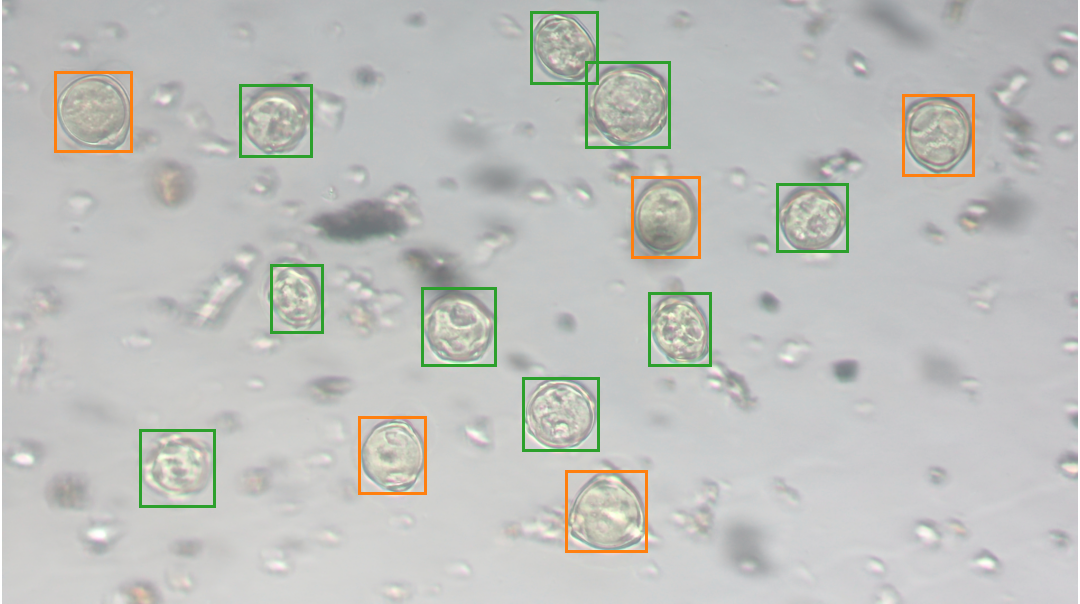
\includegraphics[width=0.8\textwidth]{figs/Snap-057.png}
  \caption[Dataset example]{Example from the dataset with ground truth bounding boxes drawn. The image contains two classes: \textcolor{corylus}{corylus}, and \textcolor{alnus}{alnus}.}\label{fig:dataset-sample}
\end{figure}

Three microscope slides have been imaged using a digital optical microscope producing a set of 701 raster images with a size of \(1080\times 1920\) pixels and three channels; red, green, and blue.
The resolution of each image is \(\SI{0.183}{\micro\metre\per\pixel}\).
Each image has been labled in collaboration with the experts to produce a valid and correct ground truths.
In total, three different species have been classified namely \textit{Poaceae}, \textit{corylus}, and \textit{alnus}, known in english as Grasses, Hazel, and Alder, respectively. An example is given in Figure~\ref{fig:dataset-sample}.

%\section{Arcitecture}\label{sec:architecture}

\section{Sharpness Measure}\label{sec:method-sharpness}
Analyzing how the sharpness of pollen grains affects detection performance requires an objective sharpness measure.
In this section we will detail how sharpness will be measured for the purpose of our analysis.
The measure is based on fourier analysis and its performance has been tested on the training data.

\subsection{Fourier analysis}
Fourier analysis describes the general method of utilizing the fourier transform to analyse the component frequensies present is some signal.
With digital images, we can look at how the brightness changes accross an image following some vector, and use this signal as the basis for our analysis.
An image contains signals in all directions so the fourier transform of an image also encodes this directionality.
Interpreting this value as a signal we can then use the fourier transform to analyse the frequency components of an image, being interpreted as a set of signals.

Using the fourier spectrum to measure sharpness follows from the realization that there is a strong relationship between the sharpness of an image in the spacial domain and the distribution of frequency components in the frequency domain.
Sharp features produce high frequencies while blur smoothes out the changes in brighness, lowering the frequencies.
Figure~\ref{fig:fourier} shows three different pollen grains, captured with progressively more blur.
If we look at their corresponding fourier spectra we can see that, as the percieved blur increases, the amount of high frequency components decrease.
In the figure, the fourier spectra are centered so the lowest frequency component lies in the middle and increases outwards.
The color map is log scaled so that the higher frequencies become visible.

\begin{figure}[htbp]
  \centering
  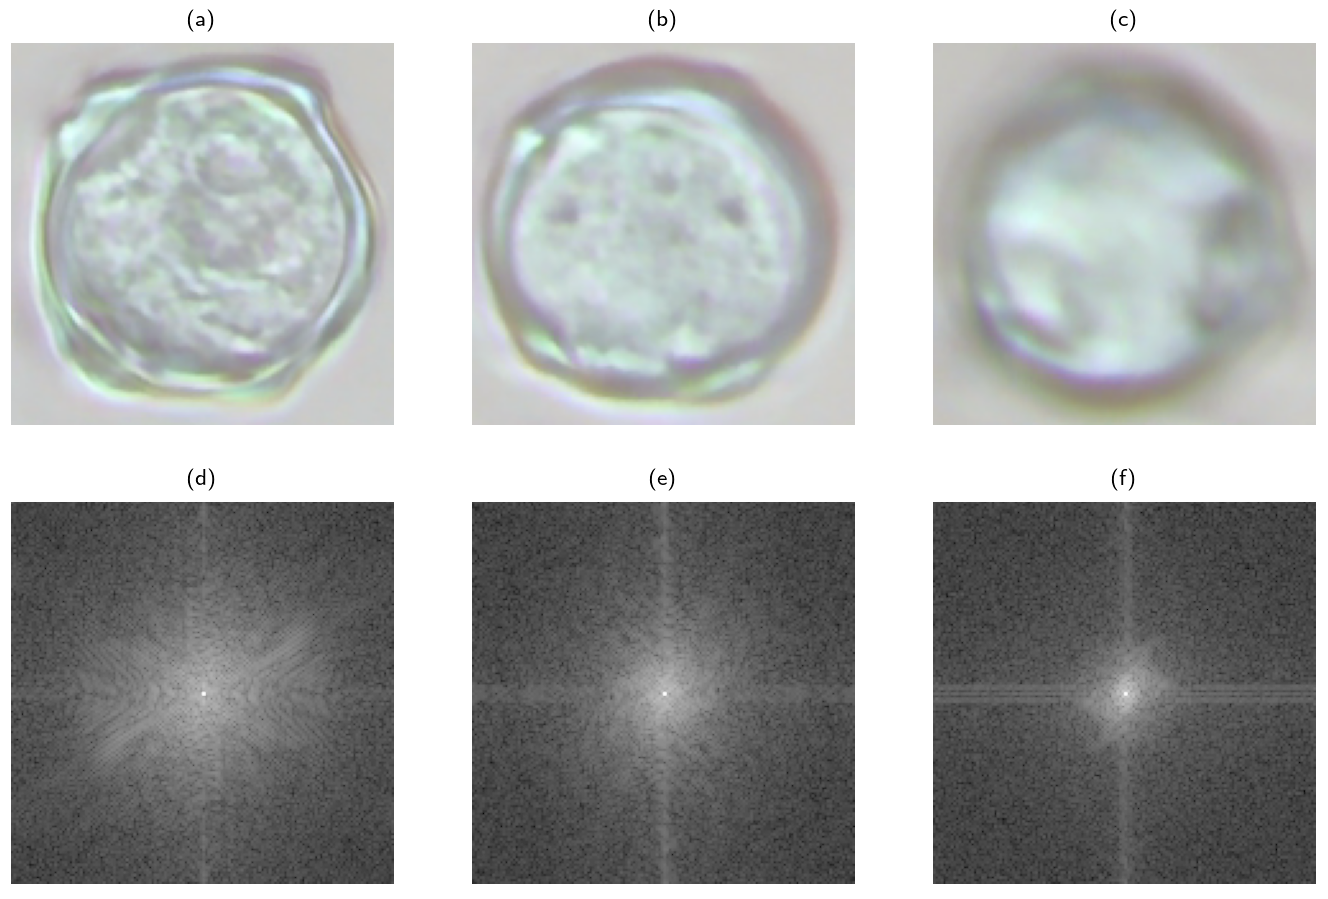
\includegraphics[width=0.8\textwidth]{figs/fourier.png}
  \caption[Fourier spectrum]{Pollen grains and their coresponding centered fourier spectrum.}\label{fig:fourier}
\end{figure}

\subsection{Measuring sharpness}
We must then decide how to encode this change in frequency distridution as a scalar sharpness measure.
\citeauthor{de2013image} propose a simple method which counts the number of components in the fourier spectrum having a value above a certain threshold.
The operation is described in Equation (\ref{eq:sharp}).


\begin{equation}\label{eq:sharp}
  \begin{split}
    \mathbf{X} = \mathcal{F}(a),\quad a\in \mathbb{Z}^{M\times N}\\
    T_H = \sum_{x\in\mathbf{X}}[x\ge\mu],\quad \mu=\frac{\max \mathbf{X^{\mathrm{abs}}}}{1000}\\
    S = \dfrac{T_H}{M\times N}
  \end{split}
\end{equation}

Here \(\mathcal{F}\) is the dicrete the fourier fransform, operationg on a input image \(a\), and \(\mathbf{X}\) only contains the magnitude of the fourier transform.
The scaling factor of the threshold value, \(\mu \), was found to produce good results on our data, without modification.

Validating the sharpness measure is an important task.
The weight of any argument made based on analysis using this measure is predicated on its soundness.
There are many different approches to this, we have chosen to compare the objective measure with subjective measurements of percieved sharpness on a subset of the training data.

\subsection{Evaluating the sharpness measure}
The basis of our evaluation is a new dataset created from a small random subset of the training examples.
Each ground truth is then given sharpness scores based on percieved sharpness and the objective measure.
Determining percieved sharpness of a pollen grain with high fidelity was found to be highly subjective and non-reproducible whith repeated independent scoring, so a simple classification was instead performed.
Images where separated into three classes representing percieved sharpness.
Figure~\ref{fig:fourier} gives examples of the classes with image (a) being the sharpest (class 3) and (c) being the blurriest (class 1).
A total of 389 pollen grains where evaluated, the distribution of their classes is given in Table~\ref{tab:sharpness}

\begin{table}[htb]
  \caption[Sharpness dataset distribution]{Distribution of classes accross the sharpness validation dataset.}\label{tab:sharpness}
  \centering 
  \begin{tabular}{lr} \toprule
    Sharpness & Frequency \\ \midrule
    1 --- blurred & 123 \\
    2 & 105 \\
    3 --- sharp & 125 \\ \bottomrule
  \end{tabular}
\end{table}

Looking at Figure~\ref{fig:sharpness} we can see a clear correlation between the mean of the distribution, and the percieved sharpness.
The overlap is to be expected, given the mapping from a continuous predictor onto a categorical label.
To further evaluate the performance of the sharpness measure, we construct a very simple statistical model, in the form of a decision tree, and test its ability to differentiate between the classes.
The model achived a test accuracy of 84.1\%.

\begin{figure}[htbp]
  \centering
  \begin{subfigure}[t]{0.49\textwidth}
    \centering
    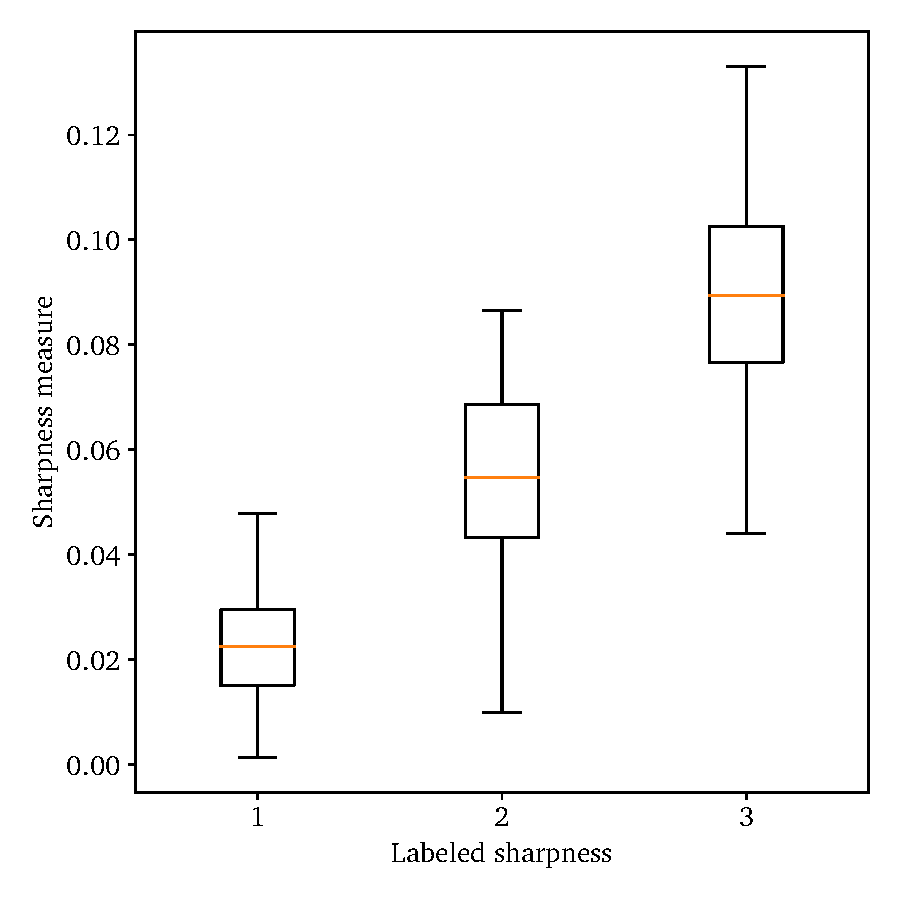
\includegraphics[width=\textwidth]{figs/box.pdf}
    \caption{Box plot}\label{fig:sharpness-box}
\end{subfigure}%
\hfill
\begin{subfigure}[t]{0.48\textwidth}
  \centering
  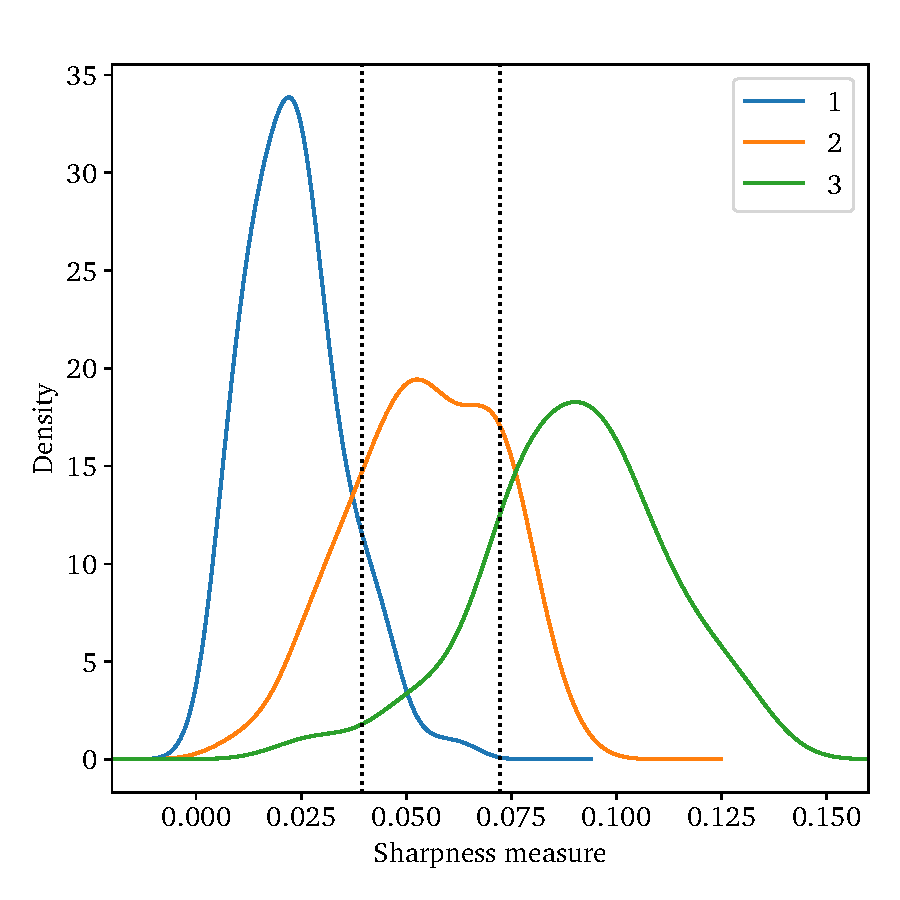
\includegraphics[width=\textwidth]{figs/qden.pdf}
  \caption{Density plot}\label{fig:sharpness-qden}
\end{subfigure}
  \caption[Sharpness measure seperability]{The sharpness measure grouped by class label. Although there is an overlap between ajacent classes, there is a clear seperation between the IQR of measured sharpness in (a). The correlation between percieved and measured sharpness is also clear.}\label{fig:sharpness}
\end{figure}
